\chapter{Bausteinsicht}
\label{sec:bausteine}
Die Bausteinsicht ist der Grundrissplan einer jeden Software. Für die Anwendung eCourse ist die Bausteinsicht in Abbildung \ref{fib:Bausteinsicht} dargestellt.
Diese Darstellung ist eine statische Zerlegung des Systems in Bausteine. Diese Ansicht ermöglicht es vor allem die Kommunikation zwischen den Entwicklern untereinander bzw. mit dem Stakeholder zu erleichtern, da sie das System abstrahiert und dadurch von der Besprechung von Implementierungsdetails entbindet

\begin{figure}[H]
\centering
\includegraphics[height=1.0\textwidth]{bausteinsicht.png}
\caption{Bausteinsicht für die Anwendung eCourse}
\label{fib:Bausteinsicht}
\end{figure}

\section{Gesamtsystem}
Durch eCourse soll es \gls{Studierende}n und \gls{Dozierende}n möglich sein Dateien untereinander auszutauschen. Ebenso sollen Verwaltungsangestellte einen Einblick in die ausgetauschten Dateien haben und verwaltende Tätigkeiten ausführen können. Diese drei Benutzergruppen greifen direkt auf die Anwendung eCourse zu. Es gibt keine weiteren Schnittstellen zu anderen Anwendungen, wie in Kapitel \ref{sec:kontext} bereits erläutert wurde. 

\section{Überblick}
Blickt man genauer in die Anwendung eCourse hinein, ergibt sich eine Aufteilung in \gls{Backend} und \gls{Frontend}.

\subsection{Frontend}
Das \gls{Frontend} beschreibt dabei den Teil der Anwendung, der näher am Nutzer liegt, es interagiert mit dem Benutzer. Es ist also die Schnittstelle zwischen Nutzer und der dahinter liegenden Logik der Anwendung. Alle drei Nutzergruppen haben Zugriff auf das \gls{Frontend}, wobei das \gls{Frontend} abhängig von der Nutzergruppe unterschiedlich mit dem Benutzer interagiert. Eine genaue Darstellung der Rechte die die jeweilige Nutzergruppe hat ist in \ref{fib:erlaubnis} zu finden.

\subsection{Backend}
Das \gls{Backend} ist dann im Gegensatz zum \gls{Frontend} die Logik hinter der Anwendung. Hier werden die Ergebnisse jeder Nutzerinteraktion berechnet. Genauere Details zum \gls{Backend} finden sich in Kapitel \ref{sec:Datenbank} und \ref{sec:Server}.

\section{Detail}

\subsection{WebInterface}
Das \gls{Frontend} besteht im Wesentlichen aus einem \gls{Webinterface}. Über eine Webseite, die als \gls{Webinterface} dient, können die Benutzer verschiedene Aktivitäten ausführen. Abhnängig davon, welcher Gruppe der Benutzer angehört sind unterschiedliche Aktionen möglich. 
Diese Aktivitäten sind in Abbildung \ref{fib:erlaubnis} dargestellt.

\begin{figure}[H]
\centering
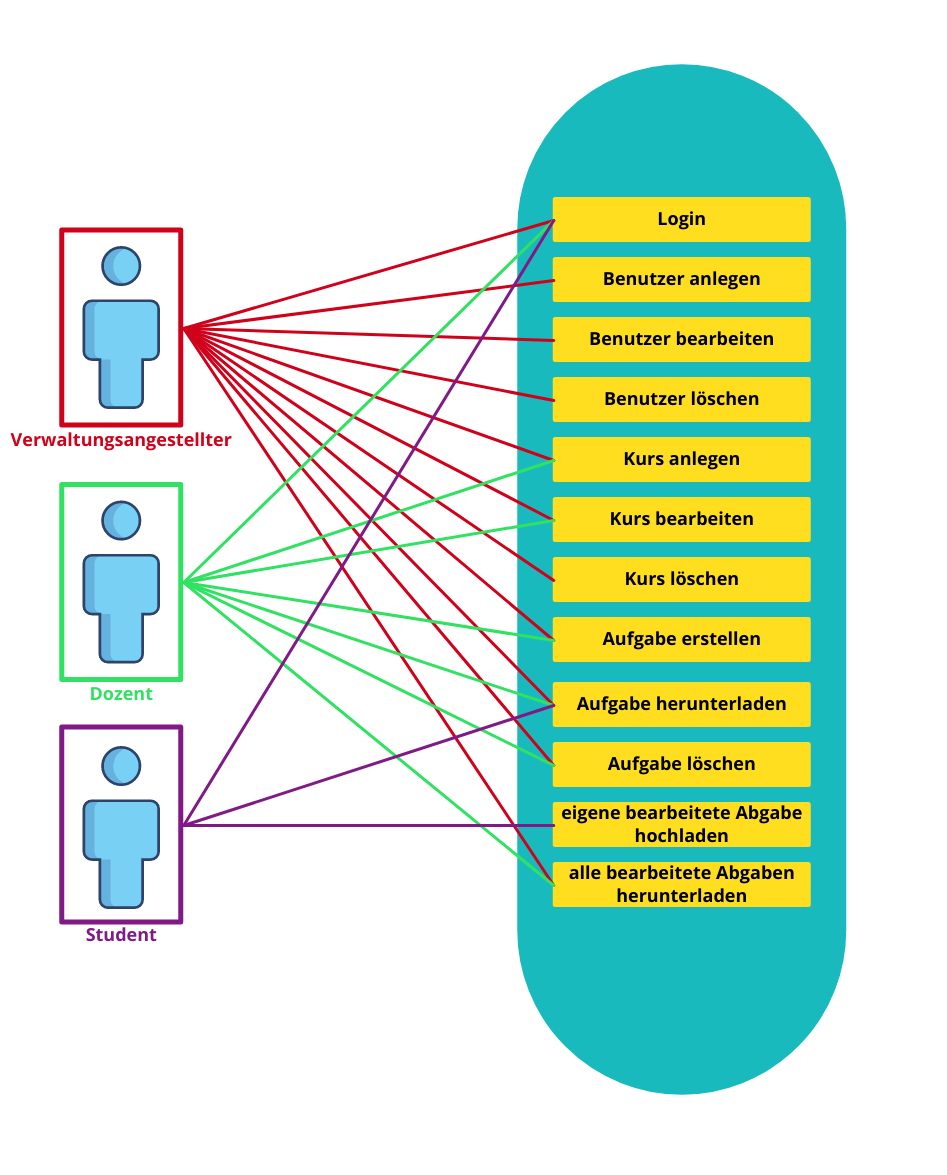
\includegraphics[height=1.0\textwidth]{erlaubnisdiagramm.png}
\caption{Bausteinsicht für die Anwendung eCourse}
\label{fib:erlaubnis}
\end{figure}

\subsection{Datenbank}
\label{sec:Datenbank}
Ein Teil des \gls{Backend}s ist die Datenbank. Diese enthält alle Daten, die während des Gebrauchs der Anwendung anfallen. \\
Im Wesentlichen stellt die Datenbank das Grundgerüst der Anwendung, auf der die Logik aufbaut.


\subsection{Server}
\label{sec:Server}
Der Server stellt dann die Logik des \gls{Backend}s. Hier werden die Daten, die in der Datenbank vorliegen verarbeitet und für die Benutzer aufbereitet. 